\documentclass{beamer}

\usefonttheme{professionalfonts} % using non standard fonts for beamer
\usefonttheme{serif} % default family is serif

\usepackage{hyperref}

%\usepackage{minted}

\usepackage{animate}

\usepackage{graphicx}

\def\Put(#1,#2)#3{\leavevmode\makebox(0,0){\put(#1,#2){#3}}}

\usepackage{color}

\usepackage{tikz}

\usepackage{amssymb}

\usepackage{enumerate}


\newcommand\blfootnote[1]{%

  \begingroup

  \renewcommand\thefootnote{}\footnote{#1}%

  \addtocounter{footnote}{-1}%

  \endgroup

}

\makeatletter

%%%%%%%%%%%%%%%%%%%%%%%%%%%%%% Textclass specific LaTeX commands.

 % this default might be overridden by plain title style

 \newcommand\makebeamertitle{\frame{\maketitle}}%

 % (ERT) argument for the TOC

 \AtBeginDocument{%

   \let\origtableofcontents=\tableofcontents

   \def\tableofcontents{\@ifnextchar[{\origtableofcontents}{\gobbletableofcontents}}

   \def\gobbletableofcontents#1{\origtableofcontents}

 }

%%%%%%%%%%%%%%%%%%%%%%%%%%%%%% User specified LaTeX commands.

\usetheme{Malmoe}

% or ...

\useoutertheme{infolines}

\addtobeamertemplate{headline}{}{\vskip2pt}



\setbeamercovered{transparent}

% or whatever (possibly just delete it)

\makeatother

\begin{document}
\title[DCEL report]{RIDIR Report}
\author[AC]{Andres Calderon}
\institute[Fall'19]{University of California, Riverside}
\makebeamertitle
\newif\iflattersubsect

\AtBeginSection[] {
    \begin{frame}<beamer>
    \frametitle{Outline} 
    \tableofcontents[currentsection]  
    \end{frame}
    \lattersubsectfalse
}

\AtBeginSubsection[] {
    \begin{frame}<beamer>
    \frametitle{Outline} 
    \tableofcontents[currentsubsection]  
    \end{frame}
}

\begin{frame}{Some tests with bigger dataset}
    \begin{itemize}
        \item Solving some performance issues with full CA\_district polygons dataset.  It was not able to finish even using the maximal number of partitions allowed (half of the number of polygons).
        \item Fixed by changing the partitions strategy.  Now, we extract the points from the polygons and create a partitioner with them.  This allows a finer and more balanced grid.
        \item Performance improves from ~200 seconds using a sample of the dataset to 5.6 seconds using the full dataset.
    \end{itemize}
\end{frame}

\begin{frame}{Test - CA dataset}
    \centering 
    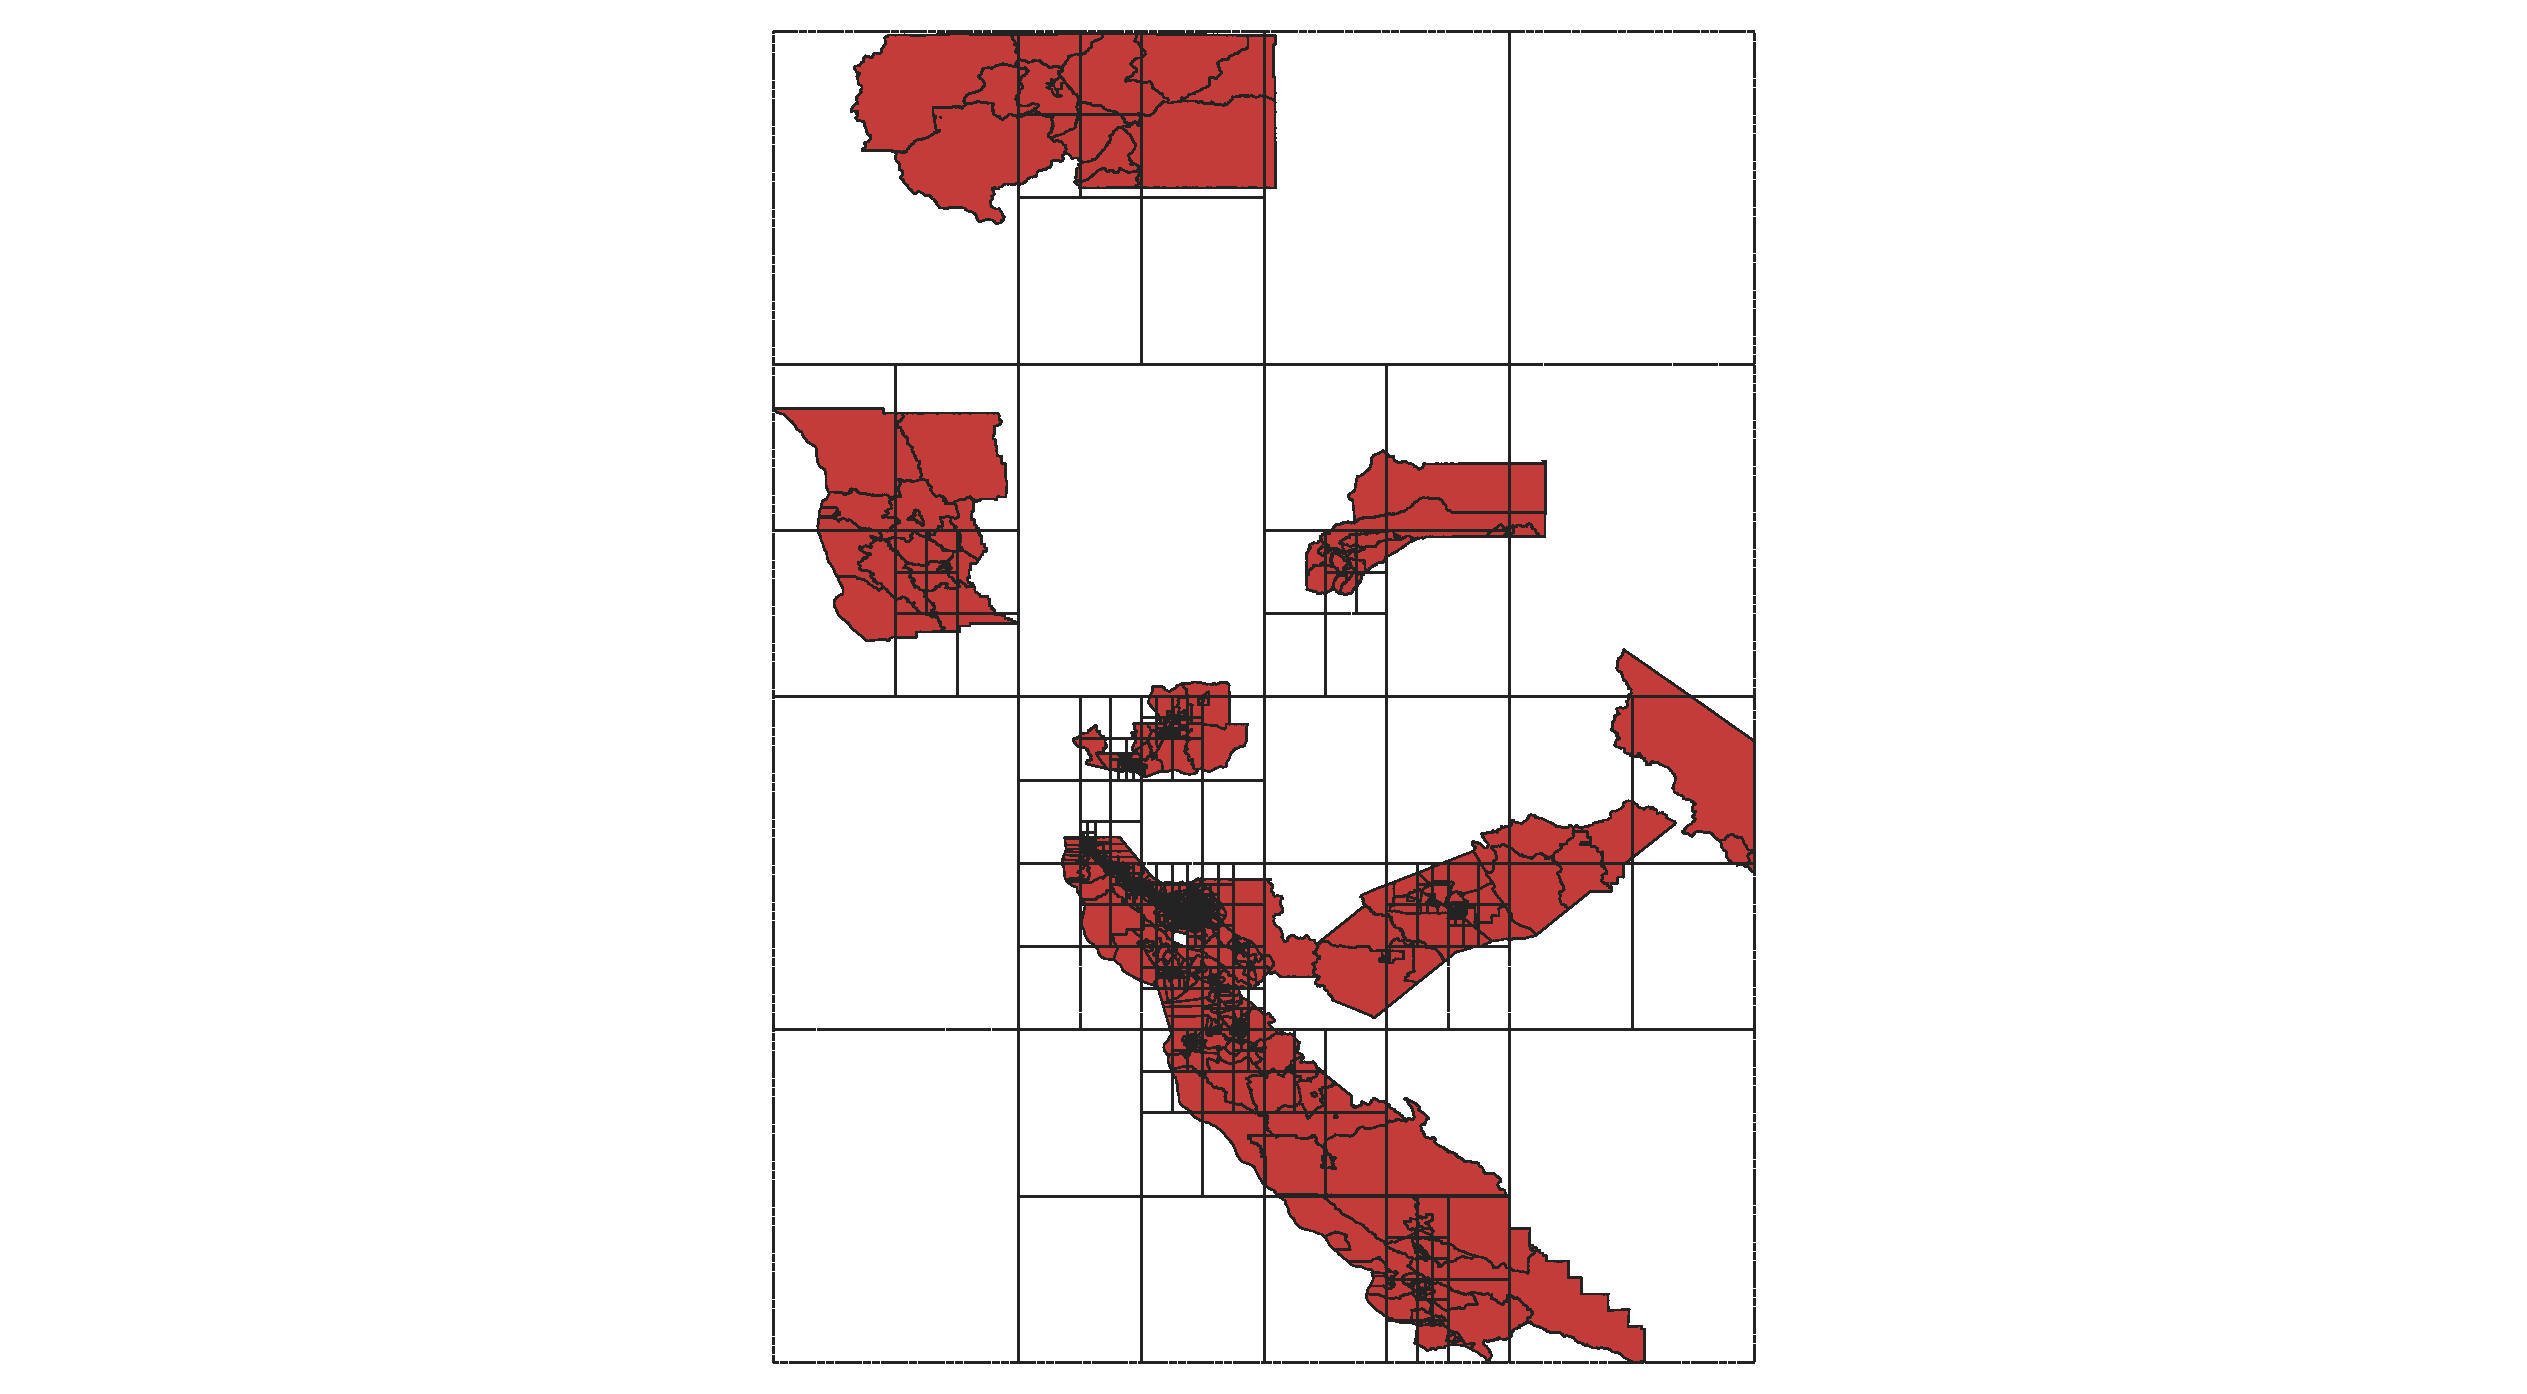
\includegraphics[width=\linewidth]{figures/CA_test} 
    \blfootnote{\tiny{Multipolygons have been removed for now}}
\end{frame}

\begin{frame}{Integrating the new changes to Merged DCEL}
    \begin{itemize}
        \item I am still working in the integration of the new changes into the code which merges independent DCELs.
        \item We are getting the correct number of results but I am dealing with an annoying bug which does not dissolve the polygons parts correctly.
    \end{itemize}
\end{frame}

\begin{frame}{Intersection Test - Phili datasets (2000 vs 2010)}
    \centering 
    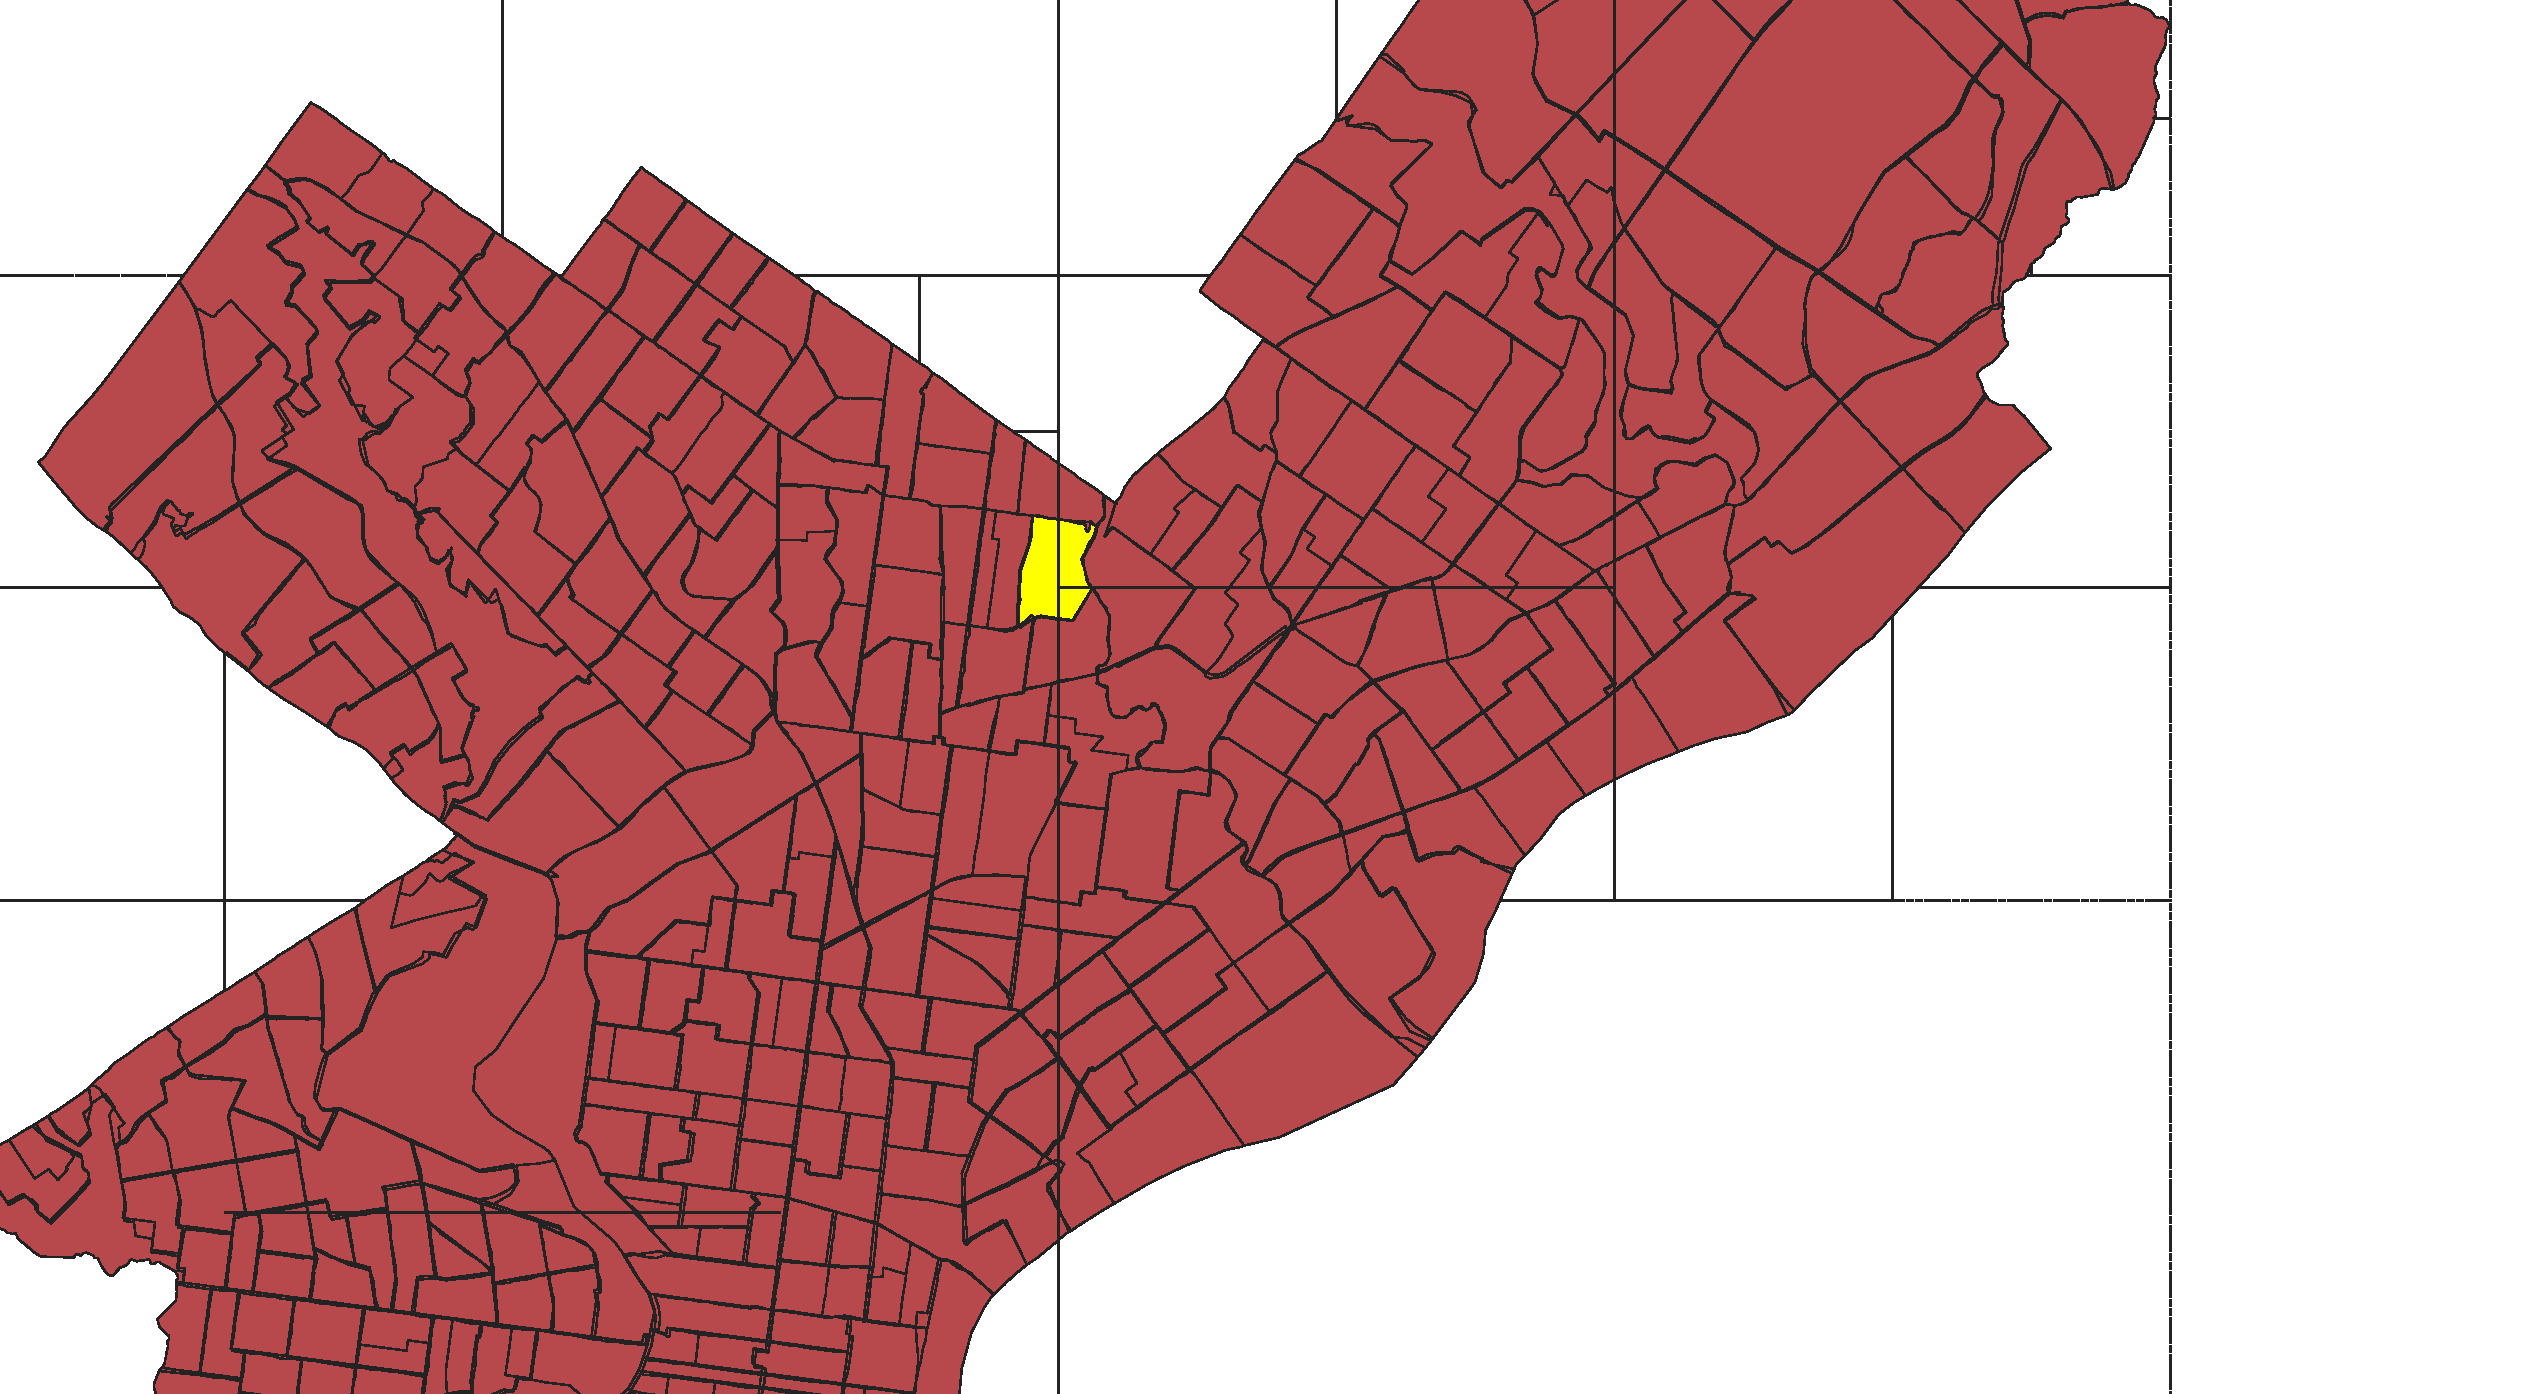
\includegraphics[width=0.9\linewidth]{figures/Phili_test} 
\end{frame}

\begin{frame}{What is next?}
    \begin{itemize}
        \item Fix bug during integration.
        \item Check support for multipolygons.
        \item Test merged DCEL with CA\_district datasets.
    \end{itemize}
\end{frame}

\end{document}
